\documentclass{article}
\usepackage{ listings} 
\usepackage{amsmath}
\usepackage{float} 
\usepackage{graphicx}
\usepackage{subcaption}
\usepackage{geometry}
\usepackage{amsthm}
\usepackage{amssymb}

\begin{document}
\title{Solution to Homework 5}
\author{Zhuo Chen and Shoeb Mohammed}
\maketitle

\newcommand{\QEDA}{\hfill\ensuremath{\blacksquare}}
\newcommand{\QEDB}{\hfill\ensuremath{\square}}

\section{Decision trees, entropy and information gain}

\subsection{}
\begin{equation}
  \label{eq:1.1}
  \begin{split}
  H\left(\frac{p}{p+n}\right) &= \frac{p}{p+n}log\frac{p+n}{p} + \frac{n}{p+n}log\frac{p+n}{n}\\
               &\leq log\left(\frac{p}{p+n}.\frac{p+n}{p} + \frac{n}{p+n}.\frac{p+n}{n}\right) \quad \text{since $log(.)$ is concave function} \\
			   &= log2 \\
			   &= 1
  \end{split}
\end{equation}
When $p=n$, the formula gives $H(S) = \frac{1}{2}log2 + \frac{1}{2}log2 = 1$.

\subsection{}
\begin{itemize}
	\item Misclassification rate for A = $\frac{1}{4}$
	\item Miscalssificationn rate for B = $\frac{1}{4}$
	\item Entropy gain model A = $\frac{3}{4}log3 - 1 \sim 0.1887$
	\item Entropy gain model B = $\frac{3}{2} - \frac{3}{4}log3 \sim 0.3113$. \\
	      This means entropy after split is lower for model B.
	\item Gini index model A = $\frac{3}{8}$
	\item Gini index model B = $\frac{1}{9}$
\end{itemize}

\subsection{}
Yes, it is possible. For an example, consider a dataset with 700 examples of class $C_1$ and 100 of class $C_2$.
If a feature splits it into two leaves $(200,200)$ and $(200,200)$; then misclassification rate is bigger.

\newpage


\section{Bagging}
\subsection{}
\begin{proof}
	
Simplifying, we get $\epsilon_{bag}(x) = \frac{1}{L}\sum\limits_{l=1}^L \epsilon_l(x)$. Thus,
\begin{equation}
  \label{eq:1.2}
  \begin{split}
	  E_{bag} &= E_X\left[\epsilon_{bag}(x)^2\right] \\
	          &= \frac{1}{L^2}E_X\left[\left(\sum_{l=1}^L \epsilon_l(x)\right)^2\right] \\
			  &= \frac{1}{L^2}E_X\left[\sum_{l=1}^L \epsilon_l^2(x) + \sum_{\substack{1\leq i,j\leq L \\ i \neq j}}\epsilon_i(x)\epsilon_i(x) \right] \\
			  &= \frac{1}{L^2}E_X\left[\sum_{l=1}^L \epsilon_l^2(x)\right]+ \frac{1}{L^2}E_X\left[\sum_{\substack{1\leq i,j\leq L \\ i \neq j}}\epsilon_i(x)\epsilon_j(x) \right] \\
			  &= \frac{1}{L^2}E_X\left[\sum_{l=1}^L \epsilon_l^2(x)\right]+ \frac{1}{L^2}\sum_{\substack{1\leq i,j\leq L \\ i \neq j}}E_X\left[\epsilon_i(x)\epsilon_j(x) \right] \\
			  &= \frac{1}{L^2}E_X\left[\sum_{l=1}^L \epsilon_l^2(x)\right] \quad \text{since $E_X\left[\epsilon_i(x)\epsilon_j(x)\right]=0$ for $i \neq j$} \\
			  &= \frac{1}{L^2} \sum_{l=1}^L E_X\left[ \epsilon_l^2(x)\right] \\
			  &= \frac{1}{L}E_{avg}
  \end{split}
\end{equation}
\end{proof}


\subsection{}
\begin{proof}
\begin{equation}
  \label{eq:1.3}
  \begin{split}
	  E_{bag} &= E_X\left[\epsilon_{bag}(x)^2\right] \\
	          &= E_X\left[\left(\sum_{l=1}^L \frac{\epsilon_l(x)}{L}\right)^2\right] \\
			  &\leq E_X\left[\sum_{l=1}^L \frac{\epsilon_l^2(x)}{L}\right] \text{using Jensen's inequality for $\lambda_i = \frac{1}{L}$; and for random variables $0\leq U\leq V$ $\implies E[U] \leq E[V]$ } \\
			  &= \frac{1}{L}\sum_{l=1}^L E_X\left[ \epsilon_l^2(x)\right] \\
			  &= E_{avg}
  \end{split}
\end{equation}
\end{proof}

\newpage

\section{Fully connected neural networks and convolutional neural networks}

\subsection{Fully connected feed-forward neural networks}

\subsubsection{Affine layer: forward}
{\footnotesize 
Testing affine\_forward function:\\
difference (should be around 1e-9):  9.76985004799e-10\\
}


\subsubsection{Affine layer: backward}
{\footnotesize
Testing affine\_backward function:\\
dx error (should be around 1e-10):  4.81624004347e-08\\
dtheta error (should be around 1e-10):  5.01568076009e-11\\
dtheta\_0 error (should be around 1e-10):  1.41109427148e-11\\
}

\subsubsection{ReLU layer: forward}
{\footnotesize
Testing relu\_forward function:\\
difference (should be around 1e-8):  4.99999979802e-08\\
}

\subsubsection{ReLU layer: backward}
{\footnotesize
Testing relu\_backward function:\\
dx error: (should be around 1e-12):  3.27563500104e-12\\
}


\subsubsection*{Sandwich layers}
{\footnotesize
Testing affine\_relu\_forward:\\
dx error:  1.94653644744e-10\\
dtheta error:  3.01172010229e-10\\
dtheta\_0 error:  3.275617042e-12\\

Testing svm\_loss:\\
loss: (should be around 9):  9.00075514465\\
dx error (should be around 1e-9):  1.40215660067e-09\\
}

\subsubsection*{Loss layers: softmax and SVM}
{\footnotesize
Testing softmax\_loss:\\
loss (should be around 2.3):  2.3026611292\\
dx error (should be around 1e-8):  8.78168746044e-09\\
}

\subsubsection{Two layer network}
{\footnotesize
Testing initialization ... \\
Testing test-time forward pass ... \\
Testing training loss (no regularization)\\
26.5948426952\\
Running numeric gradient check with reg =  0.0\\
theta1 relative error: 1.22e-08\\
theta1\_0 relative error: 6.55e-09\\
theta2 relative error: 3.57e-10\\
theta2\_0 relative error: 2.53e-10\\
Running numeric gradient check with reg =  0.7\\
theta1 relative error: 2.53e-07\\
theta1\_0 relative error: 1.56e-08\\
theta2 relative error: 1.37e-07\\
theta2\_0 relative error: 9.09e-10\\
}

\subsubsection{Overfitting a two layer network}
{\footnotesize
sgd\_solver=solver.Solver(model,data,update\_rule='sgd',\\
\qquad                  optim\_config=\{\\
\quad                    'learning\_rate': 1e-3,\\
\quad                  \},\\
\quad                  lr\_decay=0.95,\\
\quad                  num\_epochs=10, batch\_size=100,\\
\quad                  print\_every=100)\\
\quad}\\

\begin{figure}[H]
\centering
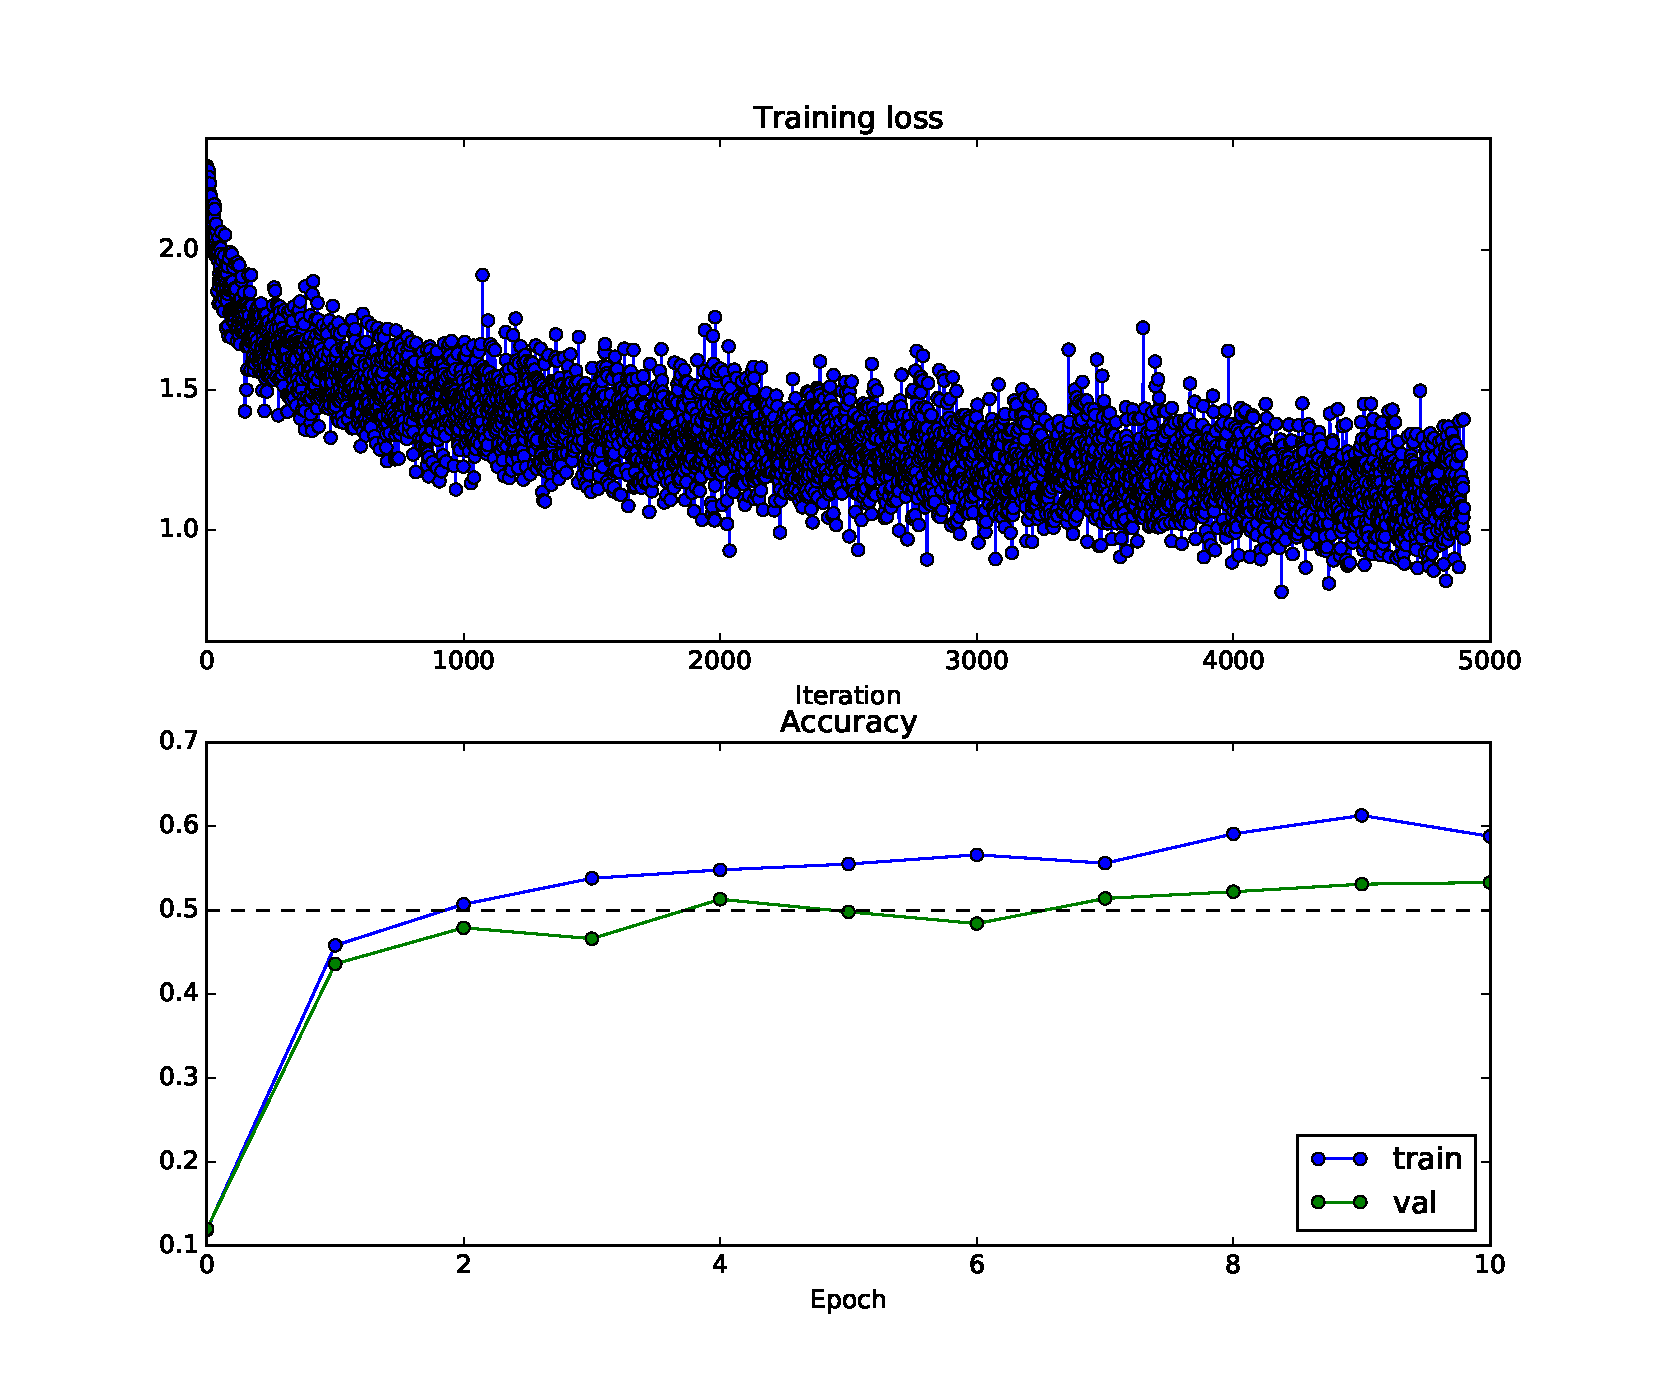
\includegraphics[width=0.5\linewidth]{./figure_3_1_6}
\caption{overfitting a two layer network}
\label{fig:3_1_6}
\end{figure}

\subsubsection{Multilayer network}
{\footnotesize
Running check with reg =  0\\
Initial loss:  2.30057347606\\
theta1 relative error: 6.88e-07\\
theta1\_0 relative error: 2.57e-08\\
theta2 relative error: 1.26e-06\\
theta2\_0 relative error: 3.01e-09\\
theta3 relative error: 7.15e-08\\
theta3\_0 relative error: 1.15e-10\\
Running check with reg =  3.14\\
Initial loss:  7.24807573499\\
theta1 relative error: 3.26e-08\\
theta1\_0 relative error: 2.89e-08\\
theta2 relative error: 6.90e-06\\
theta2\_0 relative error: 1.19e-08\\
theta3 relative error: 2.38e-08\\
theta3\_0 relative error: 3.83e-10\\
}

\subsubsection{Overfitting a three layer network}
{\footnotesize
weight\_scale = 1e-2\\
learning\_rate = 1e-2\\
\vdots\\
(Iteration 31 / 40) loss: 0.080666\\
(Epoch 16 / 20) train acc: 0.960000; val\_acc: 0.189000\\
(Epoch 17 / 20) train acc: 1.000000; val\_acc: 0.165000\\
(Epoch 18 / 20) train acc: 1.000000; val\_acc: 0.181000\\
(Epoch 19 / 20) train acc: 1.000000; val\_acc: 0.181000\\
(Epoch 20 / 20) train acc: 1.000000; val\_acc: 0.177000\\
}

\begin{figure}[H]
\centering
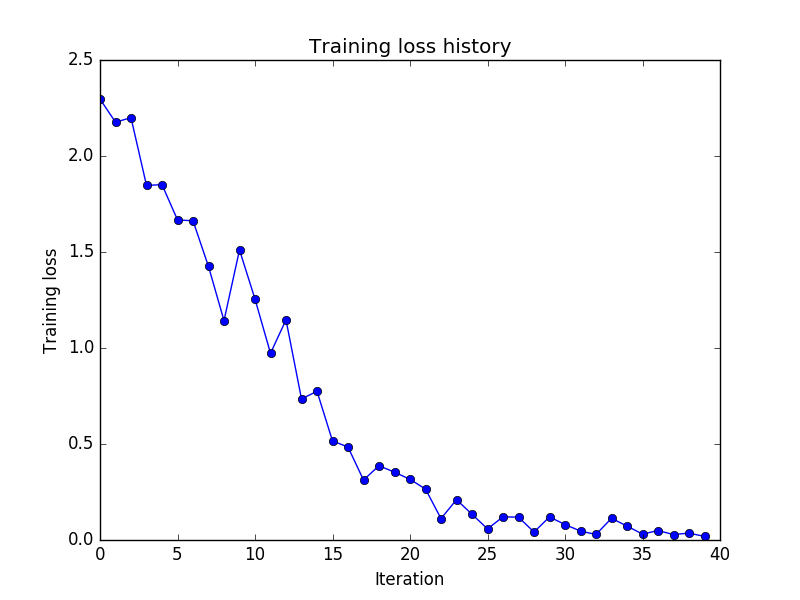
\includegraphics[width=0.5\linewidth]{./figure_3_1_8}
\caption{overfitting a three layer network}
\label{fig:3_1_8}
\end{figure}

\subsubsection{Overfitting a five layer network}
On our laptop, with the particular parameters, didn't notice a significant slowdown.
{\footnotesize
learning\_rate = 1e-2\\
weight\_scale = 5e-2\\
\vdots\\
(Epoch 10 / 20) train acc: 0.980000; val\_acc: 0.131000\\
(Iteration 21 / 40) loss: 0.180435\\
(Epoch 11 / 20) train acc: 1.000000; val\_acc: 0.128000\\
(Epoch 12 / 20) train acc: 1.000000; val\_acc: 0.130000\\
(Epoch 13 / 20) train acc: 0.980000; val\_acc: 0.121000\\
(Epoch 14 / 20) train acc: 1.000000; val\_acc: 0.135000\\
(Epoch 15 / 20) train acc: 1.000000; val\_acc: 0.141000\\
(Iteration 31 / 40) loss: 0.037009\\
(Epoch 16 / 20) train acc: 1.000000; val\_acc: 0.142000\\
(Epoch 17 / 20) train acc: 1.000000; val\_acc: 0.140000\\
(Epoch 18 / 20) train acc: 1.000000; val\_acc: 0.141000\\
(Epoch 19 / 20) train acc: 1.000000; val\_acc: 0.138000\\
(Epoch 20 / 20) train acc: 1.000000; val\_acc: 0.139000\\
}

\begin{figure}[H]
\centering
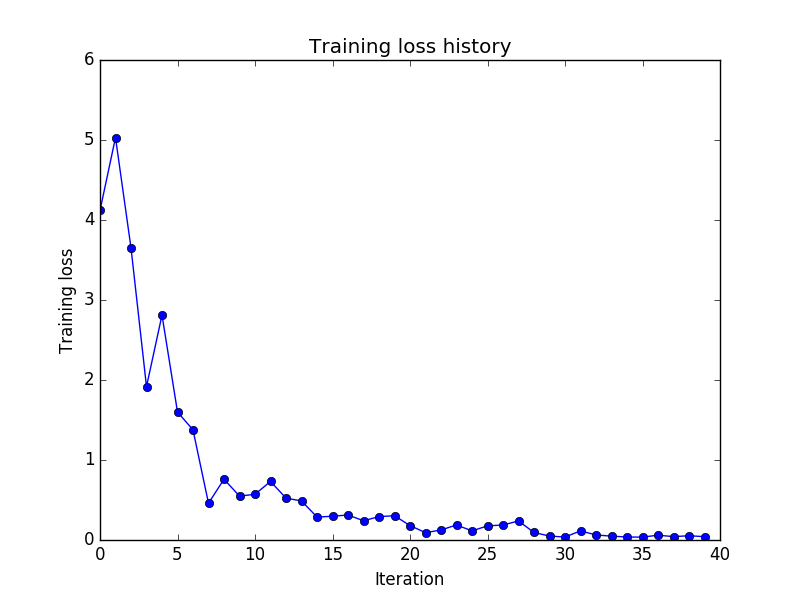
\includegraphics[width=0.5\linewidth]{./figure_3_1_9}
\caption{overfitting a five layer network}
\label{fig:3_1_9}
\end{figure}


\subsubsection{SGD+Momentum}
{\footnotesize
next\_theta error:  8.88234703351e-09\\
velocity error:  4.26928774328e-09\\
}

\begin{figure}[H]
\centering
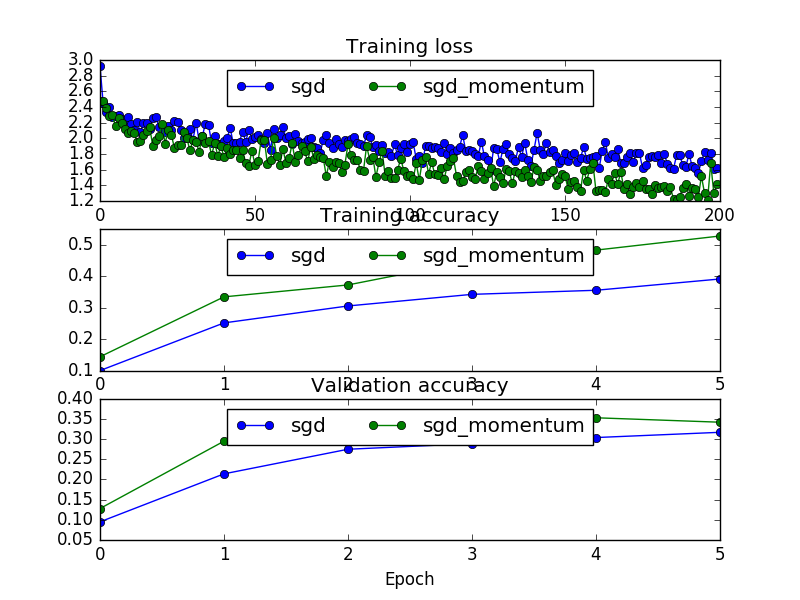
\includegraphics[width=0.5\linewidth]{./figure_3_1_10}
\caption{SGD+momentum converges faster}
\label{fig:3_1_10}
\end{figure}

\subsubsection{RMSProp}
{\footnotesize
Test rmsprop\\
next\_theta error:  9.52468751104e-08\\
cache error:  2.64779558072e-09\\
\\
Test adam\\
next\_theta error:  1.13988746733e-07\\
v error:  4.20831403811e-09\\
m error:  4.21496319311e-09\\
\\
running with adam\\
\vdots\\
(Epoch 4 / 5) train acc: 0.532000; val\_acc: 0.378000\\
(Iteration 161 / 200) loss: 1.255240\\
(Iteration 171 / 200) loss: 1.213894\\
(Iteration 181 / 200) loss: 1.206805\\
(Iteration 191 / 200) loss: 1.078037\\
(Epoch 5 / 5) train acc: 0.602000; val\_acc: 0.389000\\
\\
runnning with rmsprop\\
\vdots\\
(Epoch 4 / 5) train acc: 0.495000; val\_acc: 0.338000\\
(Iteration 161 / 200) loss: 1.452923\\
(Iteration 171 / 200) loss: 1.495491\\
(Iteration 181 / 200) loss: 1.300043\\
(Iteration 191 / 200) loss: 1.495532\\
(Epoch 5 / 5) train acc: 0.522000; val\_acc: 0.352000\\
}

\begin{figure}[H]
\centering
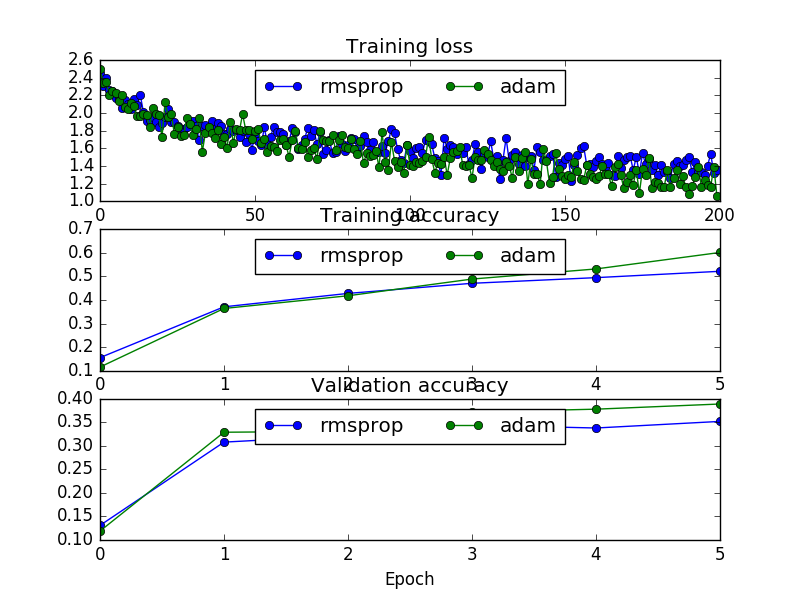
\includegraphics[width=0.5\linewidth]{./figure_3_1_11}
\caption{RMSProp and adam}
\label{fig:3_1_11}
\end{figure}

\subsubsection{Training a fully connected network for the CIFAR-10 dataset}
{\footnotesize
num\_epochs = 15\\
batch\_size = 100\\
update\_rute = adam\\
learning\_rate = 5e-4\\
\vdots\\
(Iteration 7291 / 7350) loss: 1.517843\\
(Iteration 7301 / 7350) loss: 1.358143\\
(Iteration 7311 / 7350) loss: 1.385554\\
(Iteration 7321 / 7350) loss: 1.652732\\
(Iteration 7331 / 7350) loss: 1.717880\\
(Iteration 7341 / 7350) loss: 1.258574\\
(Epoch 15 / 15) train acc: 0.587000; val\_acc: 0.520000\\
}
\begin{figure}[H]
\centering
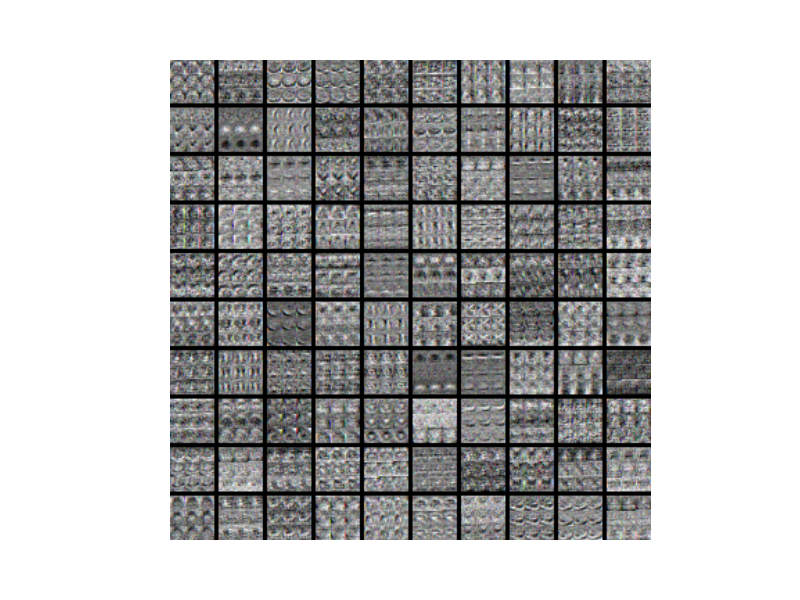
\includegraphics[width=1.0\linewidth]{./figure_3_1_12}
\caption{first level weights: Training a fully connected network for the CIFAR-10 dataset}
\label{fig:3_1_12}
\end{figure}

\subsection{Convolutional neural networks}

\subsubsection{Convolution: naive forward pass}
{\footnotesize
Testing conv\_forward\_naive\\
difference:  2.21214765759e-08\\
}

\subsubsection{Convolution: naive backward pass}
{\footnotesize
Testing conv\_backward\_naive function\\
dx error:  3.8095645582e-09\\
dtheta error:  2.06384371241e-09\\
dtheta0 error:  1.75061765296e-11\\
}

\subsubsection{Max pooling: naive forward pass}
{\footnotesize
Testing max\_pool\_forward\_naive function:\\
difference:  4.16666651573e-08\\
}

\subsubsection{Max pooling: naive forward pass}
{\footnotesize
Testing max\_pool\_backward\_naive function:\\
dx error:  1.89289002555e-11\\
}

\subsubsection*{Fast layers}
{\footnotesize
Testing conv\_forward\_fast:\\
Naive: 0.186149s\\
Fast: 0.047950s\\
Speedup: 3.882143x\\
Difference:  1.08780209978e-12\\
\\
Testing conv\_backward\_fast:\\
Naive: 0.051805s\\
Fast: 0.018498s\\
Speedup: 2.800583x\\
dx difference:  2.22406937467e-12\\
dtheta difference:  1.01018341604e-13\\
dtheta0 difference:  1.82671908726e-15\\
\\
Testing pool\_forward\_fast:\\
Naive: 0.022964s\\
fast: 0.005683s\\
speedup: 4.040863x\\
difference:  0.0\\
\\
Testing pool\_backward\_fast:\\
Naive: 0.920883s\\
speedup: 38.093981x\\
dx difference:  0.0\\
}

\subsubsection*{Convolutional sandwich layers}
{\footnotesize
Testing conv\_relu\_pool\\
dx error:  1.61462396734e-07\\
dtheta error:  3.47841604703e-10\\
dtheta0 error:  5.0140326449e-11\\
\\
Testing conv\_relu:\\
dx error:  6.41173584371e-09\\
dtheta error:  1.14601136903e-09\\
dtheta0 error:  1.85216131307e-10\\
}

\subsubsection{Three layer convolutional neural network}

\subsubsection*{Testing the CNN: loss computation}
{\footnotesize
Initial loss (no regularization):  2.30258719511\\
Initial loss (with regularization):  2.50906848795\\
}

\subsubsection*{Testing the CNN: gradient check}
{\footnotesize
theta1 max relative error: 9.317318e-03\\
theta1\_0 max relative error: 1.084071e-05\\
theta2 max relative error: 2.227715e-02\\
theta2\_0 max relative error: 9.350040e-08\\
theta3 max relative error: 5.010592e-05\\
theta3\_0 max relative error: 1.805620e-09\\
}
\subsubsection*{Testing the CNN: overfit small data}

{\footnotesize
\vdots
(Iteration 18 / 20) loss: 0.617444\\
(Epoch 9 / 10) train acc: 0.830000; val\_acc: 0.212000\\
(Iteration 19 / 20) loss: 0.580641\\
(Iteration 20 / 20) loss: 0.491107\\
(Epoch 10 / 10) train acc: 0.880000; val\_acc: 0.221000\\
}
\begin{figure}[H]
\centering
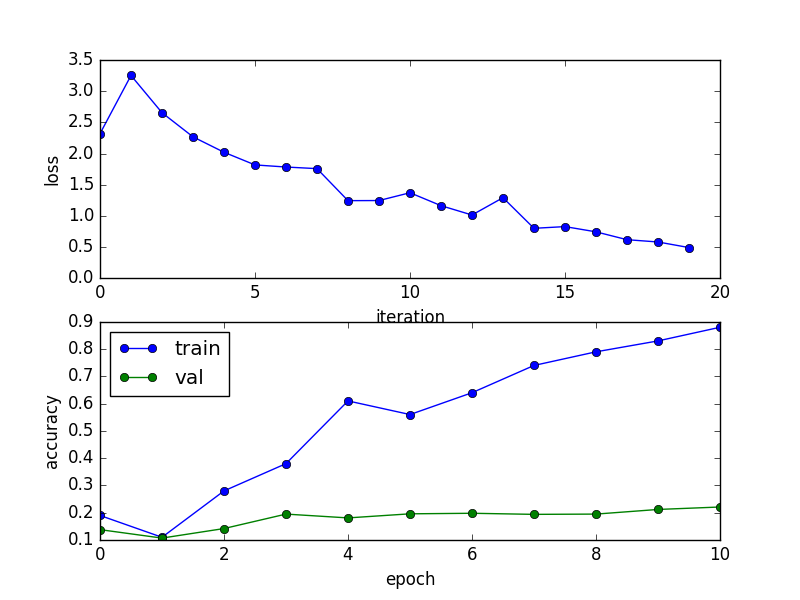
\includegraphics[width=1.0\linewidth]{./figure_3_2_5}
\caption{testing CNN: overfit small data}
\label{fig:3_2_5}
\end{figure}

\begin{figure}[H]
\centering
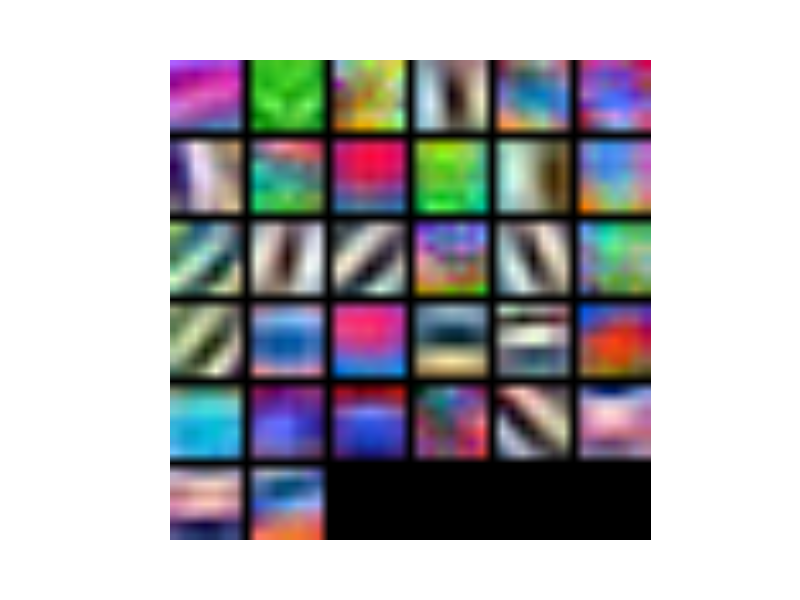
\includegraphics[width=1.0\linewidth]{./figure_3_2_5b}
\caption{testing CNN: visualizing first layer covolutional filters}
\label{fig:3_2_5}
\end{figure}

\subsubsection{Train the CNN on the CIFAR-10 data}

\end{document}
